%%%%%%%%%%%%%%%%%%%%%%%%%%%%%%%%%%%%%%%%%%%%%%%%%%%%%%%%%%%%%%%%%%%%%%%%
\chapter{Object Detection}
%%%%%%%%%%%%%%%%%%%%%%%%%%%%%%%%%%%%%%%%%%%%%%%%%%%%%%%%%%%%%%%%%%%%%%%%
\textcolor{red}{(Sloučit s úvodem?)}

Object detection aims to locate objects in a given image and assign them to their class (also called category or label). The task can be broken down into three steps: informative region selection, feature extraction, and classification. In the first step, the method has to determine regions to which we apply the feature extraction. The extracted semantic representation for each selected region is then used to predict the target's class. 

Traditionally, engineers had to hand-craft feature extractors using algorithms such as SIFT \cite{sift}, SURF \cite{surf}, or HOG \cite{hog}. These methods are combined with well-established classification algorithms such as Support Vector Machines (SVM) \cite{svm}. Since this approach needs manual designing, it can be very demanding.

Deep learning methods introduced an end-to-end learning approach, which means that the model only takes a given set of annotated images to learn to detect key features, localize the objects, and classify them. So the hard work is done mainly by the model itself. This approach outperforms the traditional pipelines by a significant margin with respect to illumination and viewpoint changes \cite{outperforming}. For illustrative comparison see Figure \ref{fig:comparison}. We describe deep learning in detail in the following Chapter \ref{deep_learning_chapter}.

\begin{figure}[h]
    \centering
    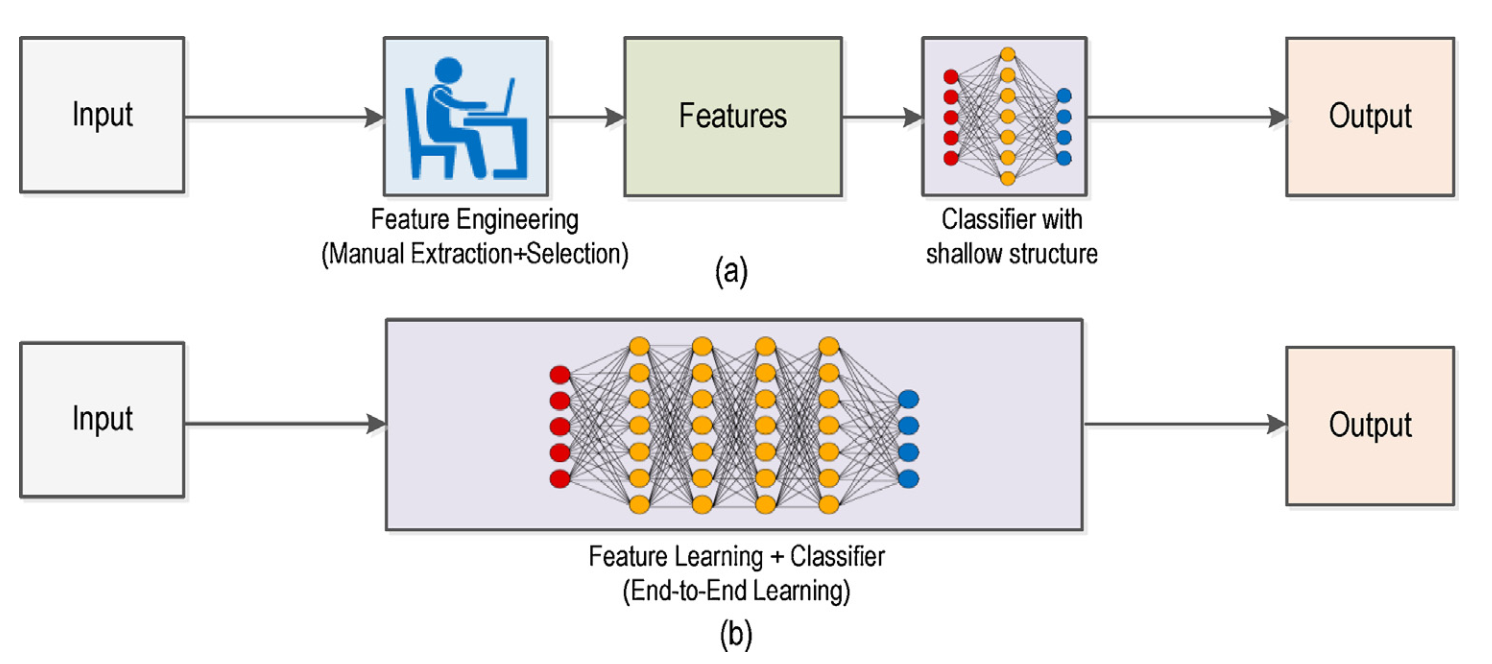
\includegraphics[width=\linewidth]{Sources/Figures/comparison.png}
    \caption{Comparison of: (a) Traditional approach and (b) Deep learning approach. Adapted from \cite{comparison_illustration}. \todo{Zmenit obrazek, clovek mate.}}
    \label{fig:comparison}
\end{figure}

